
\chapter{Supplementary description of the Reach-to-Grasp experiment}
\label{sec:R2G_suppl}

\section{Experimental apparatus}
\label{sec:experimental_apparatus}

The experimental apparatus was composed by a target object, a table switch, a visual cue, and a reward system. On each recording day, the monkey was seated in a custom-made primate chair and placed in front of that apparatus. The non-working arm of the monkey was loosely restrained in a semi-flexed position. To control the home position of the working hand between the reach-to-grasp movements, the table switch which was installed close to the monkey at waist level, 5cm lateral to the mid-line, needed to be pressed down. The target object was a stainless steel rectangular cuboid (40mm x 16mm x 10mm) rotated 45 degrees around the horizontal axis and pointing towards the monkey (\cref{fig:task_trialscheme}a). It was located 13cm away from the table switch at 14cm height. The posterior end of the object was attached through a low-friction horizontal shuttle to a counterweight hidden inside the apparatus, which was used to set the object load. The object load was set to one of two possible values to define the force type (LF and HF) needed for pulling the object in each trial by deactivating and activating an electromagnetic weight resting below the counterweight inside the apparatus. When activated, it attached to the counterweight and increased overall weight from usually 100gram to 200gram, which corresponds roughly to a pulling force of 1Newton and 2Newton for LF and HF, respectively. 

As already mentioned, the object was equipped with six sensors which monitored the monkey's reach-to-grasp behavior. Four force sensitive resistance sensors (FSR sensors) on the object surface provided continuous measurement of the grip forces applied on the object sides by the index and middle finger, as well as the thumb. The different activation patterns of these four FSR sensors, in particular the different placement of the thumb (see \cref{fig:task_trialscheme} a), were used to detect online if the correct grip type was performed. An additional FSR sensor was installed between the object and its counterweight. This FSR sensor was used to measure the horizontally applied force needed to oppose the corresponding object load. Due to the low, but still existing friction of the object moving inside the horizontal shuttle, the measured force signal of this sensor is not perfectly proportional to the horizontal force needed to lift the opposed object load, but sufficient to distinguish between LF and HF settings (cf., example in bottom right panel of \cref{fig:overview_data_l_1} and \cref{fig:overview_data_n_1}). The horizontal displacement of the object over a maximal distance of 15mm was measured by a hall-effect (HE) sensor. All sensors of the object are summarized in \cref{tab:overview_sensors}. The visual cue system, composed of a square of five LEDs (size 10 x 10 mm), was located just above the target object and used to instruct the monkey about the requested behavior. While the central yellow LED was used to warn the monkey that a trial had started, the four red corner LEDs were used to code separately the grip and the force type for the requested trial type of each trial. In this context the illumination of the two left, the two right, the two bottom, or the two top LEDs coded for SG, PG, LF, or HF, respectively (see \cref{fig:task_trialscheme} b for illustration). The reward system consisted of a bucket filled with apple sauce and equipped with a feeding tube and a pump allowing to deliver on demand the reward (few drops of the apple sauce) to the monkey (\cref{fig:task_trialscheme} a).

\begin{table}[]
\footnotesize
\centering
\begin{tabular}{llllll}
\hline
sensor & channel ID & label     & located at       & activated by          & used to identify  \\ \hline
FSR 1  & 137        & GF pr1    & object’s top     & index finger’s touch  & PG type           \\ 
FSR 2  & 138        & GF side1  & object’s left    & middle finger’s touch & SG type           \\ 
FSR 3  & 139        & GF pr2    & object’s bottom  & thumb touch           & PG type           \\ 
FSR 4  & 140        & GF side2  & object’s right   & thumb touch           & SG type           \\ 
FSR 5  & 141        & LoadForce & object’s spring  & object loading        & pulling force     \\ 
HE     & 143        & Displ     & object's shuttle & object displacement   & object’s position \\ \hline
\end{tabular}
 \caption[Overview of six objects sensors to monitor and control the monkey's behavior]{Overview of the six object sensors used to monitor and control the monkey's behavior. The first four force sensitive resistance (FSR) sensors are used to monitor the applied grip type. They are located on the surface of each object side and are activated by the touch of the corresponding monkey's finger. The fifth FSR is located at the spring counterbalancing the pull resistance of the object and is used to measure the pulling force applied by the monkey. The hall-effect sensor (HE) is located along the low-friction shuttle of the object and used to measure the position of the object. The signals of all sensors are saved in the ns2 with the stated channel ID and label (cf. \cref{fig:cerebus_system}).}
 \label{tab:overview_sensors}
\end{table}

\subsection{Behavioral control system}
\label{sec:behavioral_control_system}

The core of the behavioral control system is a custom-made Virtual Instrument (VI) in LabView that controls the digital event sequence and the requested behavior of each trial in a recording. A digital event reflects hereby the activation or deactivation of a physical device of the experimental apparatus. In this context, the LabView VI is responsible to activate and deactivate the LEDs of the visual cue system, the reward pump, and the electromagnet. The latter is not controlled by a digital event, but by an analog square signal that switches the magnet on or off. To control the requested behavior, the LabView VI monitors the monkey's manipulation of the table switch and the target object. The table switch as well as all sensors of the target object produce continuous analog signals that are digitized by the NI converter card and fed into the LabView VI of the setup computer (see \cref{fig:scidata_setup_overview} computer 2). The square signal of the table switch is then online reinterpreted as digital activation or deactivation event. \cref{fig:task_trialscheme} c displays a schematic diagram on how the physical devices of the experimental apparatus are connected to the setup computer and controlled and monitored by the LabView VI. We will now describe a typical execution of the LabView VI during a recording session in more detail. 

The possible trial types were set to SG-LF, SG-HF, PG-LF, and PG-HF, alternating with equal probability randomly in sequence between trials. Once the settings of the overall task were defined, the LabView VI was started to repetitively run and control the event sequence and behavior for each trial during the recording session. 

Each single trial was run and controlled as follows: 

The LabView VI only started a trial when the monkey deactivated the table switch by pressing and holding it down (home position, \cref{fig:task_trialscheme} a, left). This required not much muscle activity, but simply the weight of the monkey's hand on top of the smooth-running switch. If the table switch was deactivated, the LabView VI internally initiated a trial with a short time delay (TS-ON). In parallel, the program picked randomly one of the possible trial types (e.g., SG-HF) and activated or deactivated the electromagnet accordingly to fit the chosen load force of the object (e.g., activated for HF). To inform (or warn) the monkey that a new trial has started, the central LED was illuminated 400ms after the trial was initiated by the program (WS-ON). Four hundred ms after WS-ON the grip type was revealed to the monkey by illuminating the corresponding corner LEDs of the chosen trial type (CUE-ON, e.g., left LEDs for SG-ON). The LEDs of this first cue were turned off again after 300ms (CUE-OFF). The CUE-OFF was followed by a 1000ms preparatory delay at the end of which the monkey was informed about the upcoming force type by again illuminating the corresponding corner LEDs of the chosen trial type (GO-ON, e.g., top LEDs for HF-ON). This second cue also served as a GO signal for the monkey to initiate the movement which was registered by the activation of the table switch (SR-ON) when the monkey released it after a variable reaction time (RT). The execution of the movement was composed of reaching, grasping, pulling and holding the object in the position window for 500ms. The LabView VI controlled the movement execution online by checking the used grip type, the object displacement and the hold time. For checking the grip type, the grasp of the object was registered by small deflections of the FSR surface sensor signals caused by the monkey's fingers. A FSR sensor was registered as activated if the deflection surpassed a predefined threshold. The pattern of activated FSR sensors was then used by the LabView VI to control if the monkey performed the requested grip type. This meant, in particular, to check for SG and PG, if the FSR sensor on the right (GF side2), or on the bottom (GF pr2) of the object was activated by the monkey's thumb, respectively (see \cref{fig:task_trialscheme} a, middle and right). The other 2 sensors that measured force from the index and middle fingers for the 2 grip types (GF side1, and GF pr1) were not controlled online. If the correct grip was detected, the grip cue was illuminated again as a positive feedback. To check the object displacement, the LabView VI measured if the deflection of the HE sensor signal of the object was within the two defined position thresholds (4 and 14mm). The time point at which the displacement signal surpassed the lower threshold was used by the LabView VI to define the estimated start of the holding period (HS) online. If the object remained within the position window for 500ms after the HS was set, LabView activated the reward pump which provided the monkey with a drop of apple sauce as reward for a successful trial. The time until the reward pump was deactivated again by LabView was proportional to the duration of the object hold in the position window, with a maximum duration and with this a maximum amount of reward for a 500ms holding period. With this mechanism, both monkeys rapidly learned to hold the object at least 500ms in nearly all trials. In parallel to the deactivation of the reward pump, LabView turned off all LEDs to indicate that the running trial ended (WS-OFF). The monkey was allowed to release the object at its own pace as soon as it received the reward. A new trial sequence was started by LabView (TS-ON) as soon as the monkey returned to the home position (new deactivation of the table switch).

An abort of the described trial sequence by LabView (error trial) was triggered by the following three scenarios: (i) the monkey released the table switch before the GO cue, (ii) the wrong grip type was registered, and (iii) the object was not pulled and held long enough in the position window. In case one of these scenarios were registered by LabView the trial was aborted. For monkey L, the LabView VI provided additionally a negative feedback when aborting a trial by flickering all LEDs three times. 

As displayed in \cref{fig:task_trialscheme} c. the behavioral control system was connected to the NSP of the Cerebus DAQ system to store the trial event sequence and the monkey's behavior of each trial in a recording along with the neural data registered by the neural recording platform. For this, the analog signals of the sensors of the target object were copied from the NI connector block to the analog input port of the Cerebus System NSP via DC coupled BNC cables and connectors. In the NSP they were digitized with a 16-bit resolution at 0.15 mV/bit and a sampling rate of 1kHz and saved in the ns2 file under the channel ids listed in \cref{tab:overview_sensors}. All digital or digitized events that register the activation and deactivation of the table switch, the LEDs of the cue system, and the reward pump, as well as the internally generated digital trial start event (TS-ON) were coded as a 8-bit binary signal (see \cref{tab:bit_translation}) and transferred via the NI connector block to a 16-bit DB-37 input port of the NSP where they occupy the first 8 digits (remaining digits are set to 1). In the NSP the now 16-bit binary signal of each event was stored in its decimal representation and with its corresponding time point in the nev file (see \cref{tab:bit_translation} and \cref{fig:cerebus_system}).


\subsection{Neural recording platform}
\label{sec:neural_recording_platform}
The recording of the neural signals was performed using a neural recording platform with components produced by Blackrock Microsystems (Salt Lake City, UT, USA, www.blackrockmicro.com). The platform consisted of the multi-electrode Utah array, a headstage, and a Cerebus data acquisition (DAQ) system. The latter is composed of a Front-End Amplifier, a real-time Neural Signal Processor (NSP) and the control software, Central Suite (version 4.15.0 and 6.03.01 for L and N, respectively), running on Windows XP for L, and Windows 7 for N on the setup computer 1 (see Fig. \cref{fig:cerebus_system}). The Cerebus DAQ system was also connected to the behavioral control system via the NI connector block to save the analog behavioral data and digital trial event signals that were described in the previous section in parallel with the neural signals. All data were transmitted from the NSP via an ethernet cable to be saved first locally on the setup computer 1. After a recording day, all recordings were transferred to a data server. In the following, we will describe the function of the different components of the neural recording platform in more detail.

The implant location of the Utah array, as well as the electrode configuration of the array of each monkey was described previously (see \cref{fig:implant_locations}). The electrode identification numbers (IDs) are determined by how the electrodes of the array are wired and connected to the Cerebus Front-End Amplifier. See \cref{sec:channel_ids} for details.

The analog Blackrock headstage with unity gain (Samtec for monkey L, and Patient Cable for monkey N) was used to reduce the environmental noise. Overall, the reduction of the noise was better with the Patient Cable than with the Samtec headstage.

In the Front-End Amplifier, each of the 96 neural signals was differentially amplified with respect to the reference input of its corresponding connector bank (gain 5000) and filtered with a 1st-order 0.3Hz high pass filter (full-bandwidth mode) and a 3rd-order 7.5kHz Butterworth low pass filter. After that, the band-pass filtered neuronal signals were digitized with a 16-bit resolution at 0.25V/bit and a sampling rate of 30kHz, in the following called “raw signal”. The digitized signals were converted into a single multiplexed optical output and transmitted via a fiber-optic data link to the NSP. In the NSP the raw signals were saved in a ns5-file for monkey L and in a ns6-file for monkey N. The file format depended on the firmware and software version of the Cerebus DAQ system. In addition to the neural signals, the NSP received the analog behavioral signal recorded by the behavioral control system via the analog input port. These behavioral signals were digitized and saved with a sampling rate of 1kHz in a ns2-file. For monkey N, the ns2-file also contained a filtered and downsampled version of the raw signals, in the following called “LFP data”. To extract the LFP data, a copy of the raw data was online digitally low-pass filtered at 250Hz (Butterworth, 4th order), and downsampled to 1kHz within the NSP.

The NSP performed also an online spike waveform detection and classification controlled via the Central Suite software. The sorted spikes were used for a first online inspection of the data as well as for selecting and saving the spike waveforms for offline sorting. For this purpose the neuronal raw signals were for monkey L online high-pass filtered at 250 Hz (Butterworth, 4th order) and for monkey N band-pass filtered between 250Hz and 5kHz (Butterworth, 2nd order). Afterwards, the waveforms were detected by threshold crossing (manually set). These waveforms were then sorted by requesting the signal from identified neurons to follow through up to five hoops set by the user (all individually for each channel). To get an overview of the quality of the data during the recordings, the sorted waveforms were displayed in the online classification window provided by Central Suite.

The thresholds (one for each channel) for the spike waveform detection were not modified during a session and were saved in the nev-file for each session along with all other settings (e.g. filter setting etc) and configurations of Central Suite. The data and corresponding settings of Central Suite can also be inspected offline using the Blackrock software CentralPlay even in the absence of the Blackrock hardware system. Each time the high-pass filtered signal passed the threshold, a snippet of 1.6ms (48 samples) for monkey L and 1.3ms (38 samples) for monkey N was cut and saved as potential spike waveform. The snippet was cut with 10 sample points before threshold crossing and 38 or 28 points after for monkey L or N, respectively. Waveforms identified as potential single units (online sorted spikes) were labeled with IDs from 1 to 16. Unsorted waveforms were labeled with ID 0. These potential spike waveforms were saved together with their respective time stamps in the nev-file. Due to the high number of electrodes, online spike-sorting was moderately reliable. We therefore decided to re-sort spiking activity offline on each channel using the Plexon Offline Spike Sorter (Plexon Inc, Dallas, Texas, USA, version 3.3, for details see \cref{sec:data_preprocessing}). Results of offline sorting were saved in a copy of the original nev-file with an updated file name. 

All data files (nev, ns5/6, ccf) were saved on disk and backed-up on a data server at the end of the recording sessions. The information collected here are partly taken from \citep{Riehle_2013, Zehl_2016}.


\subsection{Origin of the channel IDs}
\label{sec:channel_ids}

The neuronal signal inputs to the Front-End Amplifier were grouped into four banks (A-D or 0-3) from which only the first 3 were used. Each bank consists of a male header with 34 pins of which 32 were the neuronal signal input channels. The other two channels served as reference and ground, respectively. In Central Suite, the identification (ID) number of each electrode of the array is defined by the position on the input bank and pin of the Cerebus Front-End Amplifier. For this Central Suite multiplies the bank ID (0, 1, 2, or 3) with the number of pins for neural signal input channels (32) and adds the ID of the pin the electrode is connected to (cf. ID conversion in \cref{fig:cerebus_system}). The electrode wiring of the Utah array is, though, not coordinated to the input banks of the Front-End Amplifer which leads to spatially unordered electrode IDs. Nevertheless, Utah arrays are fabricated usually in the same way where the corner electrodes are unconnected leading to a default (unordered) electrode ID configuration (cf. electrode configuration of monkey N in \cref{fig:implant_locations}). If in the fabrication process one of the corner electrodes was registered to be of significantly higher quality than any other electrodes of the grid, the corner electrode was connected instead and thereby changed the corresponding electrode configuration (cf. electrode configuration of monkey L in \cref{fig:implant_locations}). This led to the different ID sequences of the arrays for monkey L and N (see \cref{fig:implant_locations}). To facilitate the comparison of results between arrays with different electrode configurations, we assigned new IDs that reflect the spatial organization of the array. For this we used as reference the lower left corner electrode, when the connected wire bundle is showing to the right. These fabrication-independent, connector-aligned IDs increase linearly from bottom left to top right, line by line. They are also shown in \cref{fig:implant_locations} d as gray numbers in the array sketch, which thereby provides the mapping of the Blackrock IDs to the connector-aligned IDs. 

\begin{figure}
 \centering
 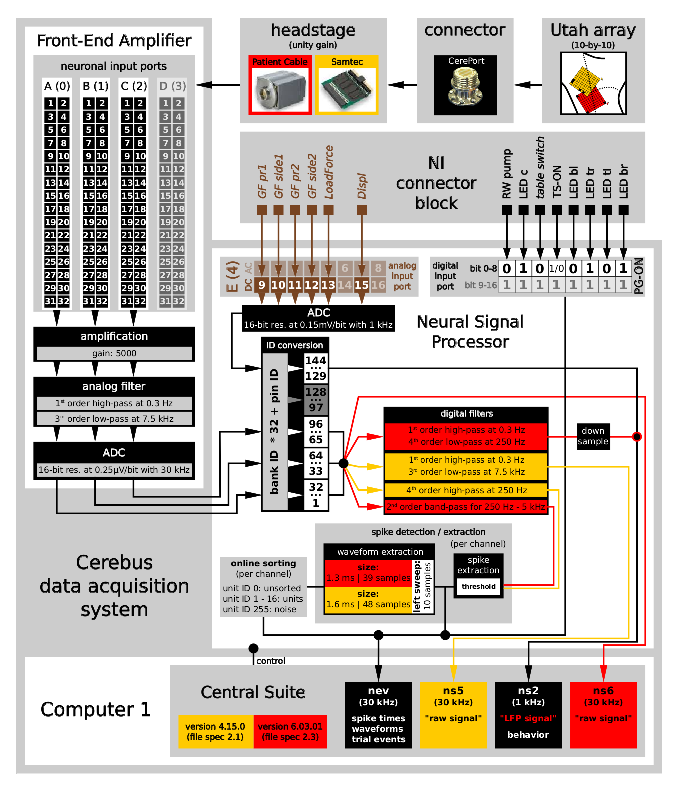
\includegraphics[width=0.7\textwidth]{./figures/scidata_figures/cerebus_system}
 \caption[Sketch of the components related to the recording of the neuronal signals]{Sketch of the components related to the recording of the neuronal signals. Data were recorded
using a Utah array, which was linked via its connector (CerePort) to a headstage (Samtec or Patient Cable) with a unity gain. From there the neural signals were transferred to the Cerebus Front-End Amplifier, where they were amplified, filtered and digitized. The digitized signals were converted into a single multiplex optical output and sent via a fiber-optic data link to the Neural Signal Processor (NSP), which is controlled by the Cerebus control software (Central Suite). Within the NSP the time points and waveforms of potential spikes were extracted online from a correspondingly processed copy of the neural signals and saved in the nev file. Simultaneously, the continuous raw signals (sampled at 30 kHz) were saved in the ns5 (for monkey L) or ns6 file (for monkey N). In parallel to the neural signals the NSP received also the digital trial events produced by the LabView VI, and the analog signals of the object’s sensors via the NI connector block of the behavioral control system. While the digital trial events were saved along with the extracted potential spikes in the nev file,
the analog signals of the sensors were digitized and saved in the ns2 file. For monkey N, a filtered and downsampled version of the neural signals (0.3–250 Hz at 1 kHz) was also saved in the ns2 file. Components and settings specific to monkey L and N are indicated by yellow and red, respectively.}
\label{fig:cerebus_system}
\end{figure}

A visual summary of the available data is given in \cref{fig:overview_data_l_1} and \cref{fig:overview_data_l_2}  for monkey L, and \cref{fig:overview_data_n_1} and \cref{fig:overview_data_n_2} for monkey N. The first of these figures shows the sequence of trials as well as selected raw recorded time series, spike trains, unit wave forms, and behavioral signals for one particular trial. The second of these figures contrasts parallel neuronal data across channels in a specific trial with neuronal data across trials in a specific channel.


\section{Data Preprocessing}
\label{sec:data_preprocessing}

After the recordings, a number of preprocessing steps (pre in the sense of before the actual upcoming data analysis, but being the post-processing after the recording) were performed as described below. This includes (i) the translation of the digital events from their binary codes set by the DAQ system to a human-readable format putting the events in context of the expected executed trial event sequence, (ii) the offline detection of behavioral trial events and object load force from the analog signals recorded by the sensors of the target object, and (iii) the offline spike sorting.

\subsection{Translation of digital events to trial events }

\cref{tab:bit_translation} lists the 8-bit combinations that were sent by LabView to the Experimental Apparatus to control the behavior. Following a binary to decimal conversion, they were saved as event codes (\cref{tab:bit_translation}) during the experiment along with their time stamps in the .nev file. In the first preprocessing step, these event codes were translated to a human-readable format and put into context of an expected trial event sequence. The validation against the latter was used to identify incomplete, correct and error trials. Error trials were further differentiated into error types (e.g., grip error). This digital event translation and interpretation (cf. \cref{tab:bit_translation}) performed automatically within the reach-to-grasp loading routine. 

Translation table of the 8 bits to the event codes and their behavioral meaning (labels). The 8 bits (see \cref{tab:bit_translation} for their meaning) were sent from LabView to NSP during the trial sequence (Fig. \cref{fig:task_trialscheme}). The event codes are the decimal version of the bit sequence assuming another byte with all bits set to 1 in front. The event codes are found in the .nev files with a time stamp and indicate the occurrence of a stimulus / behavioral event as indicated in the center column ('label'). Due to different versions of the LabView control program for monkey L and N (see text for details) the event codes for the same label may be different for the two monkeys. Also some event codes do not have a concrete meaning (miscellaneous) and occur sporadically in the .nev file due to a mistake in the sampling of the digital events - they have to be ignored. In the table the event codes are sorted in sequential order from top to bottom with respect to the task, i.e. their order corresponds to the sequence found in the .nev file in an successful trial. 

\subsection{Preprocessing of behavioral analog signals}

Some behavioral events such as the monkey touching the object or the onset of the object displacement by the monkey were controlled during the experiment, but their online-detected timing was approximate and not saved (see details in section \cref{sec:behavioral_control_system}). However, these events can be relevant for data analysis and they were thus computed offline from the analog signals of the four FSR sensors measuring the monkey's grip and the HE sensor measuring the object displacement. We implemented a custom-made Matlab \code{Event}-Detection toolbox to detect 8 specific events: the precise timing of object touch (OT) and object release (OR) from the force traces as well as the timing of displacement onset (DO) and object back to baseline (OBB) from the displacement trace, and finally the onset and offset of the plateau phase in the force and displacement traces. The plateau phase of the displacement signal indicates the timing and stability of the holding period, and its onset is used to calculate offline the hold start (HS) signal. The toolbox performed an automatic detection of these events and their timing was first approximated by threshold crossing and then fine-tuned by back-comparison of the traces with baseline level from the point of threshold crossing. Since the automatic detection was prone to errors, the trials were visually inspected one by one and the timing of the automatically detected events were manually corrected if they did not match the event times as visually identified. In addition, a Matlab script was used to inspect the load force traces in each trial to control if the actual object load corresponded to the programmed object load. This procedure ensured that the electro-magnet controlling the object load was properly activated throughout the recording session. 

\subsection{Offline spike sorting}
\label{sec:offline_spike_sorting}
The spike waveforms which were extracted and saved (in the nev file) during the recording were offline sorted using the Plexon Offline Sorter (version 3.3.3). To keep the variability in the half-manual spike sorting at a minimum, all sortings were performed by the same person (A. Riehle). The spike sorting started with loading the complete nev file of a session into the Plexon Offline Sorter. The spike sorting was performed on a duplicate of the data file to keep the original data intact. We started by joining all different waveforms extracted online from each channel separately back again into one pool and initially marked as “unsorted waveforms” in the Plexon Offline Sorter. Thereby, we ignored the result of the preliminary online waveform sorting (units 0-16 in the nev file) that was performed during the recording via Central Suite software, which served solely to extract waveforms and gain an overview of the quality of the spiking activity. For the invalidation of cross-channel artifacts (e.g., chewing artifacts) all waveforms that occurred simultaneously on a defined percentage of channels (70\%) were marked as “invalidated waveforms” in Plexon Offline Sorter. Such artifacts occurred only in the recording session of monkey L. Furthermore, a waveform rejection was performed. Thereby all waveforms of abnormally large amplitude and/or atypical shape on a channel were manually marked as “invalidated waveforms” in Plexon Offline Sorter.

The actual spike sorting was then performed on the remaining unsorted waveforms (i.e., those not marked as invalidated waveforms) individually for each channel. We used different algorithms to split these waveforms into clusters in a 2- or 3-dimensional principal component (PC) space. The dimensionality of the PC space was chosen according to the best separation. The main algorithms used were K-Means(-Scan) and Valley Seeking (chosen according to the best separation). We used a fixed threshold for outliers (a parameter to be determined in the Plexon Offline Sorter) between 1.8 (K-Means) and 2 (Valley Seeking) to get comparable sorting results. The spikes of the sorted clusters were then controlled using the inter-spike interval (ISI) distributions and the auto- and cross-correlation plots. Units were ordered manually from best to worst (assigning increasing unit IDs 1-16 in the Plexon Offline Sorter) by considering the amplitude of the waveform (the higher the better), the outcomes of the ISI analysis (no or low number of spikes with an ISI smaller than 2 ms), the correlation histograms, and identifiable cluster shapes. Waveforms in the cluster with the highest unit ID (worst) on a given channel may contain multi-unit activity. Clusters with unacceptable outcomes (completely or partly overlapping waveforms), including those with only a few spikes, left assigned as “unsorted waveforms” in Plexon Offline Sorter. This offline spike sorted nev file was saved under the file name of the original nev file with an added two-digit numeric postfix (e.g. -01). In this file, unit ID 255 contains invalidated waveforms, unit ID 0 contains the unsorted waveforms (that may enter a further cluster analysis for spike sorting), and unit IDs 1-16 contain the time stamps and waveforms of the sorted single- or multi-units (as in the Plexon Offline Sorter). Unit IDs that are considered to represent multi-unit activity are documented in the metadata. The nev file with the sorted units can be loaded again into the Plexon Offline Sorter to visualize all the sorted spikes and rework the spike sorting.

\begin{table}
\centering
\begin{tabular}{cccccc}
\hline 
\multirow{2}{*}{\textbf{monkey}} & \multirow{2}{*}{\textbf{sorting ID}} & \multirow{2}{*}{\textbf{\# SUA}} & \multirow{2}{*}{\textbf{\# MUA}} & \multicolumn{2}{c}{\textbf{\# electrodes with}}\tabularnewline
% \cline{5-6} 
 &  &  &  & \textbf{SUA} & \textbf{SUA or MUA}\tabularnewline
\hline 
\hline 
\textbf{L} & {*}-02 & 93 & 49 & 65 & 86\tabularnewline
\textbf{N} & {*}-03 & 156 & 19 & 78 & 89\tabularnewline
\hline 
\end{tabular}

\caption[Overview of offline sorted single and multi unit activity (SUA and MUA)]{Overview of offline sorted single and multi unit activity (SUA and MUA). For the recording of monkey L it was possible to sort out 93 SUAs and 28 MUAs distributed over 65 of the 96 electrodes of the Utah array, with 21 additional electrodes with further MUA recordings. For the recording of monkey N it was possible to sort out 156 SUAs and 8 MUAs distributed over 78 of the
96 electrodes of the Utah array, with 11 additional electrodes with further MUA recordings. For details on the offline spike sorting see \cref{sec:offline_spike_sorting}.}
\label{tab:datafiles_unitactivity}
\end{table}

\subsection{Code availability}
\label{sec:code_availability}

All available code required to access the data as described in \cref{sec:usage} is stored along with the datasets. The provided code includes, in particular: (i) a snapshot of the Python \software{Neo}  package (see also \cref{sec:neo}), (ii) a snapshot of the Python \software{odML} package (see also \cref{sec:odml}), (iii) the custom-written ReachGraspIO extending the \software{Neo} package, (iv) the example script shown and described in \cref{sec:usage}, (v) the code shown and described in \cref{sec:usage} demonstrating how to access the data in \software{Matlab}.

In addition to these frozen versions of the code, we recommend to use updated versions of the code to benefit from future enhancements, bug fixes and increased compatibility with future Python releases or novel applications that rely on recent versions of \software{Neo} and/or \software{odML}. Complete link collections to the two libraries can be found online\footnote{\software{Neo}, \url{http://neuralensemble.org/neo/}},\footnote{\software{odML}, \url{ and http://www.g-node.org/projects/odml}}. Importantly, both projects are hosted and version-controlled via Github\footnote{\software{Neo}, \url{https://github.com/NeuralEnsemble/python-neo}},\footnote{\software{odML}, \url{https://github.com/G-Node/python-odml}}.

\section{Data Records}

All data and metadata are publicly available via the data portal of the German Neuroinformatics Node (G-Node) of the International Neuroinformatics Coordination Facility (INCF), called GNData\footnote{GNData, \url{http://g-node.github.io/g-node-portal/}}. \cref{tab:scidata_data_overview} provides an overview of the name, size, and content of all files for each published dataset of monkey L and N. The datasets of both monkeys consist of four parts: (i) the primary data are provided as the original data files obtained from the Central Suite software stored in the data format specified by the manufacturer (in particular, nev, ns5 and ns6 format) of the neural recording platform, Blackrock Microsystems; (ii) an offline sorted version of the neural spike data (cf. \cref{sec:offline_spike_sorting}) is provided in a second nev file; (iii) metadata are provided as one file per dataset in the \software{odML} format \citep{Grewe_2011, Zehl_2016}; and (iv) a mat file is provided containing the continuous neural raw data together with the offline sorted spike data, both annotated with the corresponding metadata.

\begin{figure}
 \centering
 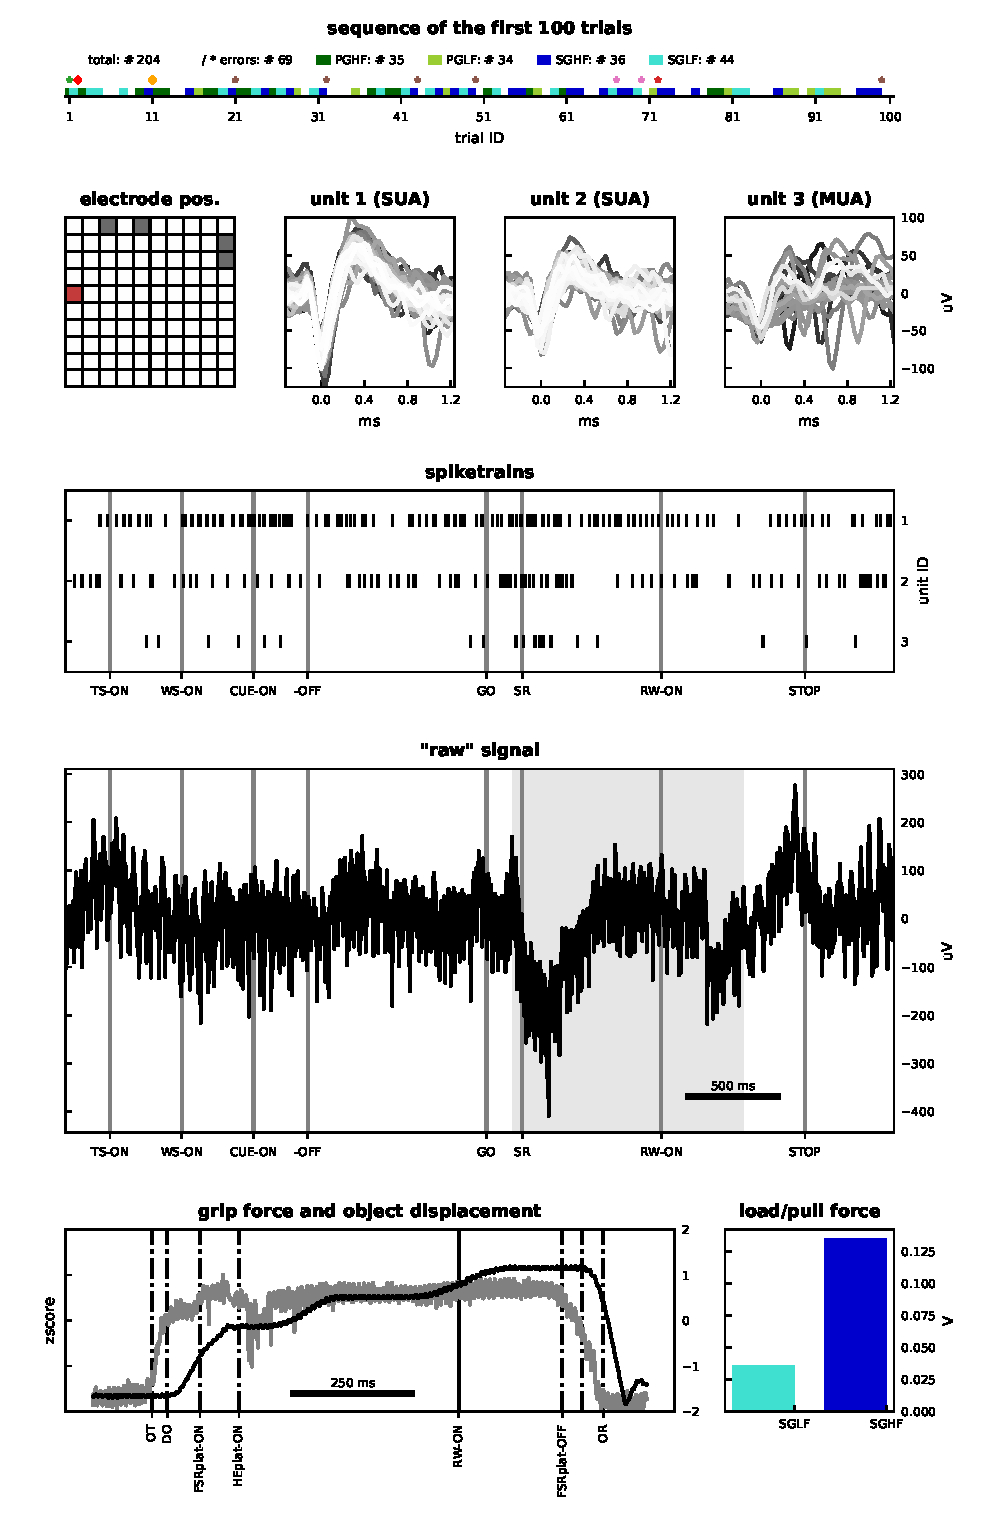
\includegraphics[width=0.8\textwidth]{./figures/scidata_figures/data_overview_1_L}
 \caption[Overview of data types contained in l101210-001]{Overview of data types contained in l101210-001. The figure displays the different data types contained in the selected dataset of monkey L. Top panel: sequence of the first 100 trials (for trial types and errors see color in legend) and the total number of trials (see \# for correct, error, trial types in legend); the red diamond marks the selected trial (trial ID: 2) for panels below; the orange diamond marks an additional trial selected to demonstrate load/pull force differences between the averaged load force signals in the bottom right panel. Asterisks indicate error trials (black asterisks: grip errors). Second row, left panel: position of selected electrode (in red) for the data plots (electrode ID: 71). Second row, remaining panels: waveforms of three units from the selected electrode. Third row: spike trains of displayed units for the selected trial. Forth row: raw signal for the selected trial; gray shaded area marks the time window corresponding to the bottom left panel. Bottom left panel: grip force (gray) and object displacement (black) signals for the selected trial. Bottom right panel: averaged load/pull force signals for the duration of the plateau of the grip force signal for the selected LF and HF trial. Important trial events are indicated as vertical lines in the corresponding data plots.}
 \label{fig:overview_data_l_1}
\end{figure}

\begin{figure}
 \centering
 \includegraphics[width=\textwidth]{./figures/scidata_figures/data_overview_2_L}
 \caption[Overview of raw signal and spike data of monkey L (l101210-001)]{Overview of raw signal and spike data of monkey L (l101210-001). Left panels: Raw signal (top) and spike data of unit IDs 1 on each given electrode (bottom) for a single trial (trial ID: 2) across a selection of electrodes. Right panels: Raw signal (top) and spike data from single unit ID 1 (bottom) across selected correctly performed trials on one electrode (electrode ID: 3). Trial events (TS-ON, WS-ON, CUE-ON, CUE-OFF, GO-ON, and RW-ON) are indicated as colored vertical lines in each plot. Trial types of selected trials in upper right panels are indicated as color (SGHF: dark blue; SGLF: cyan; PGHF: dark green; PGLF: light green)}
 \label{fig:overview_data_l_2}
\end{figure}

\begin{figure}
 \centering
 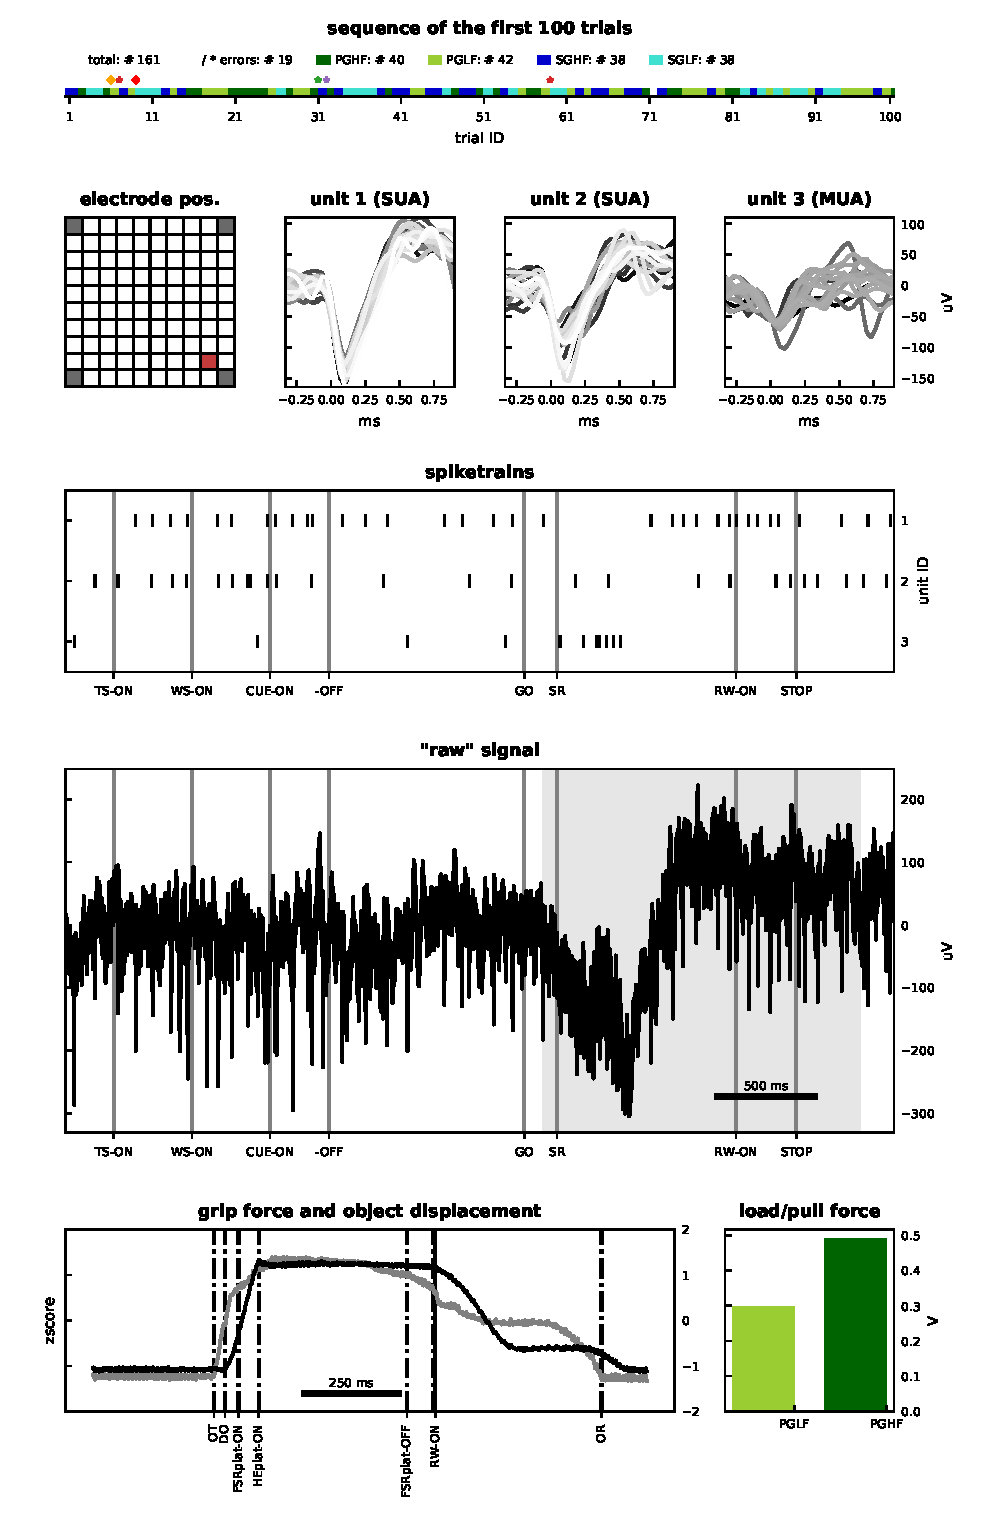
\includegraphics[width=0.8\textwidth]{./figures/scidata_figures/data_overview_1_N}
 \caption[Overview of data types contained in i140703-001]{Overview of data types contained in i140703-001. The figure displays the different data types contained in the selected dataset of monkey N. Top panel: sequence of the first 100 trials (for trial types and errors see color in legend) and the total number of trials (see \# for correct, error, trial types in legend); the red diamond marks the selected trial (trial ID: 9) for panels below; the orange diamond marks an additional trial selected to demonstrate load/pull force differences between the averaged load force signals in the bottom right panel. Asterisks indicate error trials (black asterisks: grip errors). Second row, left panel: position of selected electrode (in red) for the data plots (electrode ID: 63). Second row, remaining panels: waveforms of three units from the selected electrode. Third row: spike trains of displayed units for the selected trial. Forth row panel: raw signal for the selected trial; gray shaded area marks the time window corresponding to the bottom left panel. Bottom left panel: grip force (gray) and object displacement (black) signals for the selected trial. Bottom right panel: averaged load/pull force signals for the duration of the plateau of the grip force signal for the selected LF and HF trial. Important trial events are indicated as vertical lines in the corresponding data plots.}
 \label{fig:overview_data_n_1}
\end{figure}

\begin{figure}
 \centering
 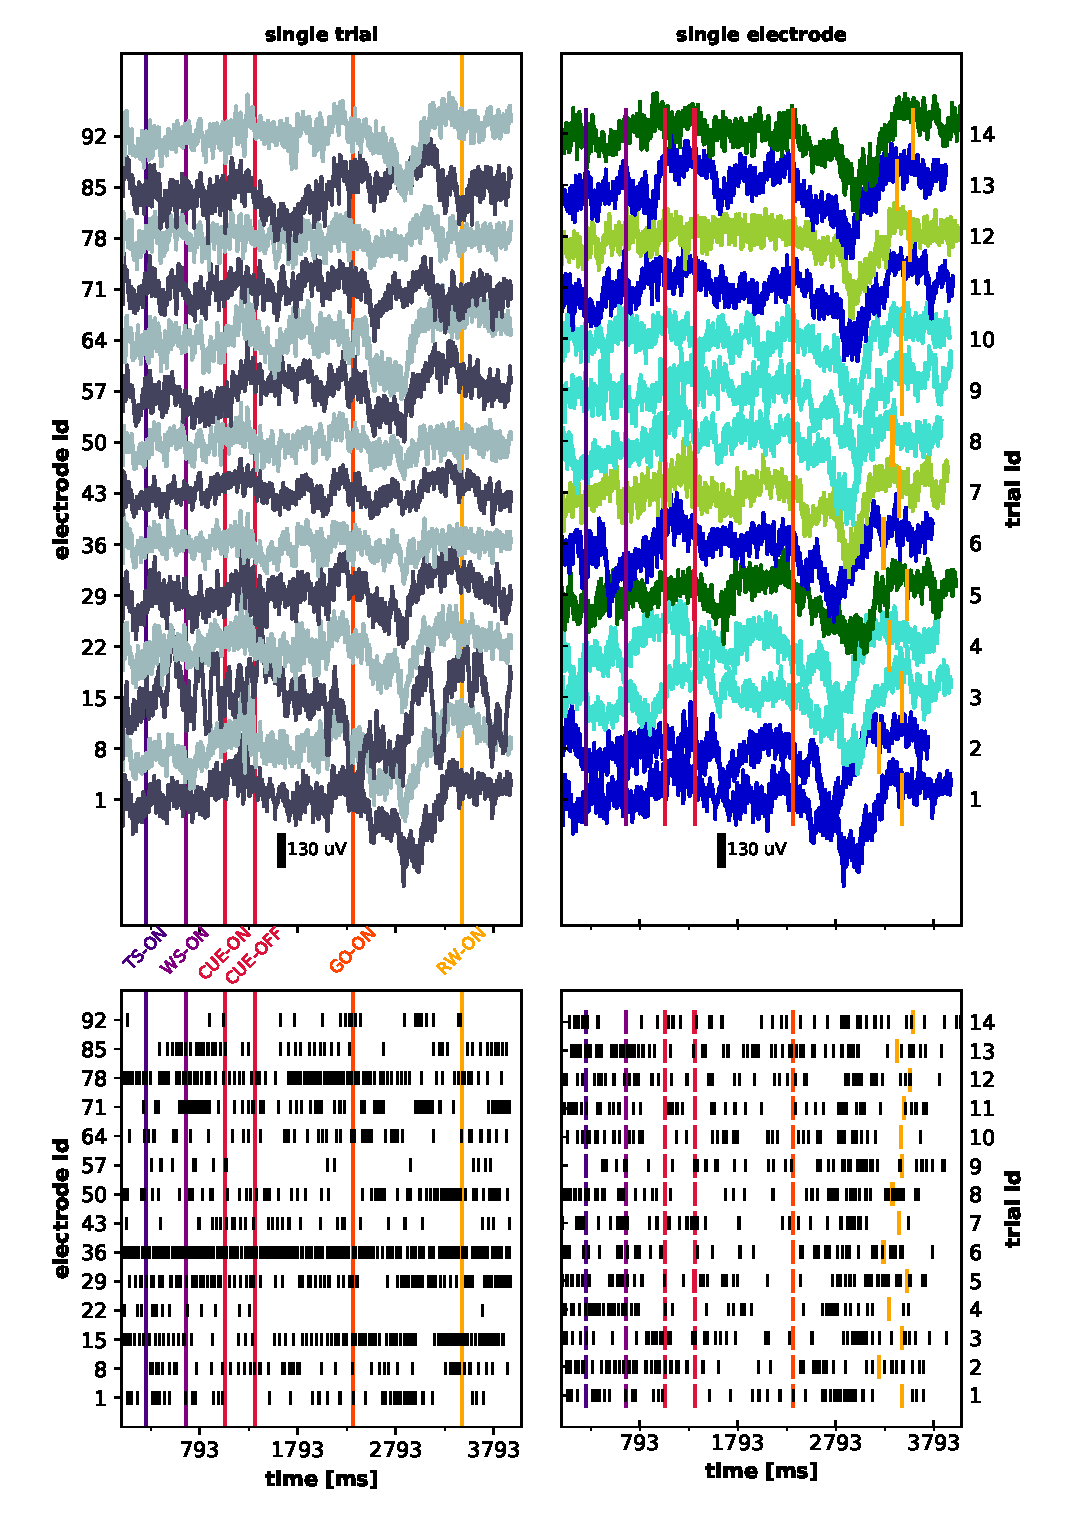
\includegraphics[width=\textwidth]{./figures/scidata_figures/data_overview_2_N}
 \caption[Overview of LFP and spike data of monkey N (i140703-001)]{Overview of LFP and spike data of monkey N (i140703-001). Left panels: LFP data (top) and spike data of unit IDs 1 on each given electrode (bottom) for a single trial (trial ID: 1) across a selection of electrodes. Right panels: LFP data (top) and spike data from single unit ID 1 (bottom) across selected correctly performed trials on one electrode (electrode ID: 1). Trial events (TS-ON, WS-ON,CUE-ON, CUE-OFF, GO-ON, and RW-ON) are indicated as colored vertical lines in each plot. Trial types of selected trials in upper right panels are indicated as color (SGHF: dark blue; SGLF: cyan; PGHF: dark green; PGLF: light green).}
 \label{fig:overview_data_n_2}
\end{figure}


Overview of recording days of the published datasets. For both monkeys, we chose to publish the first dataset (rec*-001) of the recording day. For details on the published datasets see \cref{tab:scidata_data_overview}.

The dataset l101210-001 from monkey L is the first out of 9 recording sessions conducted on Friday, December 10, 2010, while the dataset i140703-001 from monkey N is the first out of only 3 recording sessions conducted on Thursday, July 3, 2014. Both datasets were recorded in the late morning. The following recording day went on for nearly one hour and a half for monkey L, and one hour for monkey N. Although the recording from monkey N lasted with 16:43 min several minutes longer than the recording from monkey L with only 11:49 min, monkey L executed 204 trials, while monkey N only performed 160 trials in total. However, monkey L performed only ~70\% of all trials correctly, whereas monkey N successfully completed ~90\% of all trials during the recording (cf. \cref{tab:scidata_data_overview}). Nonetheless, the high percentage of error trials in monkey L are mainly caused by an too early movement onsets reflecting the eagerness, but also the nervousness of the monkey L's character. In contrast to these error types, monkey L used only 12 times the wrong grip compared to monkey N who performed an incorrect grip type 16 times during the recording. 

Overview of trials performed during the published datasets. Of the stated number of error trials, the monkey L and N used the wrong grip type in 12 and 16 trials, respectively. In the remaining error trials the monkeys initiated the movement too early. Trial types were altered randomly in the recordings which led to slightly different trial numbers for the different trial types.

For both monkeys the trial types alternated randomly between trials leading to slightly different numbers of trials with the same trial type in the each dataset (cf. \cref{tab:scidata_data_overview}). 

The quality of the spiking activity in the datasets of both monkeys was high, which allowed us to perform a relatively robust offline spike sorting with high numbers of single unit activity (SUA) distributed over all electrodes of the array (for details see \cref{tab:datafiles_unitactivity}). For details on how the offline sorting was performed and checked please have a look at \cref{sec:offline_spike_sorting} and \cref{sec:spike_data_quality}. 


\section{Technical Validation}
\label{sec:technical_validation}

In addition to the above described preprocessing steps that needed to be performed to gain more content of the raw data, some technical validations of the data also had to be conducted. These technical validations include the correction of the irregular alignment data files of the Cerebus DAQ system and a general quality assessment of the data. In order to validate the quality of the recording, a series of algorithms were applied to the data. On the one hand the quality of the LFP signals was assessed per electrode and per trial by evaluating the variance of the corresponding signal in multiple frequency bands. On the other hand the quality of the offline sorted single units (\cref{sec:offline_spike_sorting}) was determined by a signal-to-noise measure. In addition, noise artifacts occurring simultaneously in the recorded spiking activity were detected and marked. In the following, we explain these technical validation steps in detail.

\subsection{Correction of data alignment}

The ns6 file starts always 82 samples later than ns5, ns2 and nev files. This miss-alignment is caused by an error in the Blackrock recording software. However, this shift is correctly recorded in the ns6 file, and therefore will be automatically corrected in the generic \software{Neo} loading routine (cf., BlackrockIO in \cref{sec:usage} below). In addition, due to the online filter procedure, the LFP signals in the ns2 file are delayed by approximately 3.6 ms with respect to the time stamps in the nev file and the analog signal of the ns6 file. This offset was heuristically determined, documented in the metadata file, and can be automatically corrected for by the experiment-specific loading routine (cf., ReachGraspIO in \cref{sec:usage} below). Note that the time stamps of the spike times provided in the nev file correspond to start of the waveform and not to the time point of threshold crossing.

\subsection{Quality assessment}

The occurrence of noise in electrophysiological recordings is to a certain degree unavoidable and therefore needs to be carefully examined. It depends to a large extent on the quality of the headstage used to record the neurophysiological data. In our data, two different types of headstages were used for the two monkeys - the Samtec-CerePort headstage (monkey L) and the Patient Cable (monkey N). The former is much more sensitive to noise than the latter. The type of noise, its cause and appearance in the data is quite variable. Depending on the direct influence of the different types of noise on subsequent analysis methods, one needs to balance the corresponding data rejection between being very permissive and very conservative. For this reason, it is wise not remove or delete data of bad quality, but instead mark them with the judgment of a corresponding quality assessment procedure. For the here published datasets, we provide the results of our quality assessment of the electrodes, trials and spiking units along with the analysis parameters of the used procedure in the \software{odML} metadata files for each recording. The reach-to-grasp IO integrates this information by annotating the corresponding data objects in Neo. This approach not only allows the user to finally decide which data to reject for an analysis, but also provides the opportunity to provide different quality assessments of the same electrode, trial and unit at the same time. This is helpful if one considers that certain types of noise can differently contaminate signals in different frequency bands. For the here published datasets, the quality of the recorded signals was therefore separately tested for the sorted spike data and different frequency bands of the LFP data. The used corresponding procedures are described in detail below. 

\subsection{LFP data quality}

The LFP data were examined for noise in three broad frequency bands excluding the 50Hz European line noise (low: 3Hz - 10Hz, middle: 12Hz - 40Hz, high: 60Hz - 250Hz) in each session individually. The goal of the quality assessment was, first, to detect channels with a noisy signal throughout the session and, second, to detect noisy trials in the remaining “clean” channels. To do so, the analog signals of each electrode were first z-scored and filtered in the three frequency bands (low, middle, and high) using a Butterworth filter (of order 2, 3, and 4, respectively). For each frequency band the quality assessment analysis was carried out separately. The detection of noisy electrodes was performed in three steps: 

step 1 The variance of the filtered analog signal of each electrode was calculated over the complete session. 

step 2 Out of the 96 resulting variance values, outliers were identified as those values outside a user-defined range. The range was defined as follows: (i) values between a lower (e.g., 25th) and an upper (e.g., 75th) percentile (L and U), (ii) the range of acceptable values was defined by $L-w\cdot(U-L),U+w\cdot(U-L)$,where w is a user-defined whisker coefficient (e.g., w=3). 

step 3 The analog signals classified as outliers in step 2 were visually controlled by comparing them to the analog signal of an electrode with a typical variance value. If the results were either too conservative or too permissive, the detection procedure was repeated by manually adapting the chosen parameters (L, U, and w), correspondingly. 

The electrode IDs of the final outliers as well as the parameters chosen for their detection were saved in the \software{odML} metadata file of the corresponding recording and marked as noisy for the tested frequency band. 

For the remaining non-noisy electrodes, an analogous procedure was carried out afterwards to detect noisy trials. The procedure differed in one respect: the variance of the filtered analog signal was calculated for each trial on each electrode separately. At the end, the trial IDs of the identified outliers were pooled and marked as noisy for the tested frequency band on all electrodes. The marked trial IDs were saved in the \software{odML} metadata file of the corresponding recording together with the chosen analysis parameters for their detection. Note again that with this procedure a trial is marked as noisy on all electrodes as soon as it is classified as noisy on one electrode.

\subsection{Spike data quality}
\label{sec:spike_data_quality}

To test and judge the quality of the spike data, the results of the offline spike sorting were controlled first, for the signal-to-noise ratio (SNR) from the waveforms of the identified single units and second, for the occurrence of hyper-synchronous event artifacts.

1. To calculate the SNR for each identified unit in the sorting results a method introduced by \citet{Hatsopoulos_2004} was used. The SNR was defined as the amplitude (A, trough-to-peak) of the mean waveform ($<w>$) divided by twice the standard deviation of the waveform noise ($SD_{noise}$) of the defined unit (u): $SNR_{u}=A_{<w>}/SD_{noise}\cdot2$,where $SD_{noise}$ was computed by averaging the standard deviations (SDs) obtained from each sample point across the original waveforms (SD of the waveform noise adapted from \citet{Nordhausen_1996,  Suner_2005}. For all identified single units in the datasets published here, the determined SNRs ranged between $1.5$ and $12$. Corresponding to \citet{Suner_2005} the quality of the spike sorting of an identified unit is good if the SNR is above 4, is fair if the SNR ranges between 2 and 4, and is poor if the SNR ranges between 1 and 2. Units with an SNR below 1 are not considered as signals. For a conservative analysis of the spike datasets, we recommend to use only single units with a SNR of 2.5 or higher, which was our choice in e.g. \citet{Torre_2016}. The results of the SNR analysis of the performed spike sorting were saved in the \software{odML} metadata file of the corresponding recording and units were annotated accordingly. 

2. Since correlation analysis of spike data is very sensitive to cross-electrode artifacts which would produce unwanted false positive results, we controlled the sorted spike data on their original time resolution ($\delta=1/30ms$) for potential occurrence of hyper-synchronous event artifacts. For this, we computed the population histogram, i.e. the sum of the spikes across all sorted single units in the dataset in bins of $\delta=1/30ms$ (sampling resolution of the data), and detected if there were entries $\ge2$. To our surprise these hyper-synchronous spikes, which are likely to be attributed to cross-channel noise, survived the spike sorting including the cross-channel artifact removal by the Plexon Spike sorter. We indeed detected these spike artifacts during a preliminary analysis of a previous study \citep{Torre_2016}. The number of single units participating in these events ranged from 2 to over 30 and a statistical analysis showed that the frequency of their occurrence largely exceeded the expected value considering the observed population firing rate. Furthermore, a $\delta$-binned time histogram of the population spiking activity triggered around the occurrence times of the hyper-synchronous events revealed also increased spiking activity in the preceding or following bin of the event. For a conservative analysis of the spike datasets, we recommend to treat the spikes participating in a hyper-synchronous event as well as the spikes occurring within a short time interval around this event ($\scriptstyle \pm\delta$) as artifacts of unknown origin and to remove them subsequently before performing any analysis of the spike data.

In \citet{Torre_2016} we combined both quality assessments of the spike data and only considered spikes with a SNR>2.5 and additionally removed all hyper-synchronous events with $\ge2$ spikes. 


\section{Usage Notes}
\label{sec:usage}

In the following, we describe how the provided data files can be practically used in a data analysis scenario. To this end, we first briefly present the open source software libraries we recommend to use in order to access data and metadata using the Python programming language. We also demonstrate how to merge data and metadata in a common representation that facilitates data handling and analysis. Finally, we present an example program that produces a visualization of the most important data items contained in the files, and can be used as a template script for accessing the provided data. All software discussed below is provided in the code subfolder of the provided datasets, and links to the code repositories are listed in \cref{sec:code_availability}.

As outlined above, the datasets are stored in two types of files. The primary data, and the spike sorted data, are provided in the data format (in particular, the nev, ns5 and ns6 format) specified by Blackrock Microsystems, the manufacturer of the recording hardware. Second, metadata are provided as one file in the \software{odML} format \citep{Grewe_2011}. While data and metadata are provided in documented file formats (see Blackrock\footnote{Blackrock, \url{http://blackrockmicro.com/}} and \software{odML}\footnote{\url{http://www.g-node.org/projects/odml}}, respectively), the mere knowledge of the highly complex internal structure of the files is insufficient to practically make use of their content. In particular, implementations of corresponding loading routines performed from scratch by individual researchers are likely to be incoherent and error-prone. Thus, in the following we will use two community supported open-source libraries to separately load primary data and metadata into a generic, well-defined data representation. 

We chose the data object model provided by the open-source \software{Neo} library (\cref{sec:neo}) \citep{Garcia_2014} as the primary representation of the datasets (\cref{sec:neo}). \software{Neo} provides a hierarchical data structure composed of Python objects that aim to represent electrophysiological data in a generic manner. In addition, \software{Neo} provides a number I/Os that enable the user to read from (and in part, write to) a large number of open and vendor-specific file formats. In particular, \software{Neo} provides an I/O module for the file format used by Blackrock Microsystems (class BlackrockIO in file neo.io.blackrockio.py). The output of this I/O is a \software{Neo} data structure that is a faithful representation of the contents of the primary data files. For detailed information on the structure of the \software{Neo} data object model, please consult the online documentation\footnote{Neo, \url{http://neo.readthedocs.io/en/latest/index.html}}.

Here, we briefly summarize the output of the reach-to-grasp datasets obtained when calling the I/O. The \code{read\_block} method of an instantiation of the BlackrockIO returns a \software{Neo} Block object as a top level grouping object representing one recording session. In the hierarchy directly below the Block is one single \code{Segment} object spanning the complete continuous recording, and one \code{ChannelIndex} object for each of the 96 electrodes of the Utah Array (\cref{fig:implant_locations}) and each of the 6 sensor signals monitoring the target object manipulation (\cref{sec:experimental_apparatus}). The data from these 102 recording channels is each saved in one \code{AnalogSignal} object. All of these are linked to the \code{Segment} and the respective \code{ChannelIndex} object. Likewise, the spike times (and optionally, the spike waveforms) of each identified unit are saved to a \code{SpikeTrain} object. As for the \code{AnalogSignal} objects, these are linked to the \code{Segment}, and to the \code{ChannelIndex} object via a Unit object. Finally, all digital events are saved into a single \code{Event} object that lists their time of occurrences and the corresponding event IDs. Additional information from the file is provided as annotations on each individual \software{Neo} object (accessible via the annotation property of the object), in particular as annotations to the top level Block object. Note, that although this generic I/O can be used to access the raw data records, no interpretation of the file contents is given. For example, digital events are not interpreted as behavioral events, but only given as the raw numeric codes shown in \cref{fig:scidata_setup_overview}. 

In order to access the metadata stored in the \software{odML} file, we use the corresponding library API python-\software{odML} described in \citet{Grewe_2011}. In short, \software{odML} files store metadata in form of hierarchically structured key-value pairs. The \software{odML} files accompanying the provided datasets contain extensive metadata grouped into different sections describing different aspects of the experiment. A tutorial on how to work with the \software{odML} library can be found in the online documentation shipped with the library, and a more detailed description of how to manage metadata by example of the \software{odML} framework can be found in \citet{Zehl_2016}. In short, the library supports to read the content of an \software{odML} file, provides an API to navigate through the hierarchical structure, and to extract metadata of interest from the key-value pairs. Thus, the python-\software{odML} library provides a standardized way to access stored metadata records. 

As a next step, we combine the primary data and metadata in a manner that is specific to this experiment and aids the analysis process. To this end, the relevant metadata that were extracted from the \software{odML} are attached as annotations to data objects in the hierarchical \software{Neo} structure. For example, metadata information for a particular single unit originating from the spike sorting process may be attached to the \software{Neo} objects representing the sorted spike data of that unit. The task of combining the primary data and metadata is performed by a custom-written Python class named ReachGraspIO that is derived as child class from Neo's BlackrockIO class. For a full documentation of the input arguments, methods, and outputs of this class, please refer to the class documentation in reachgraspio.py. In short, invoking the \code{read\_block} method of the ReachGraspIO performs the following steps under the hood: (i) read the primary data using the \code{read\_block} method of the parent class (BlackrockIO) as described above, (ii) read the metadata using the python-\software{odML} library, (iii) interpret event data based on the digital events (e.g., detect trial start or reward), and (iv) add relevant metadata to the \software{Neo} data object using the annotation mechanism. Thus, the \software{Neo} Block object returned by the ReachGraspIO contains extensive information attached as annotations of the individual \software{Neo} objects, in particular, about whether a \code{SpikeTrain} is classified as SUA or MUA, about the spatial positioning of electrodes, or about the identities of electrodes that should be rejected. A full list of these metadata annotations can be found in the documentation of the \code{read\_block} method in the file reachgraspio.py.

In summary, for practical purposes, the resulting data structure of the ReachGraspIO hosts a complete representation of the data and a synthesis of the metadata relevant for analysis. This representation may be saved to disk in a standardized container format (e.g., .mat or HDF5), such that the exact same data and metadata context can also be accessed from other programming languages. For illustration, we provide the data object in the Matlab file format (.mat) in the folder datasets\_matlab, containing Matlab structs resembling the Python \software{Neo} objects.

In the following we demonstrate how to use the ReachGraspIO in practice in order to load and visualize the datasets. We follow the file example.py, which is contained as part of the code included with the published datasets. The goal of this program is to create a figure showing the raw signal, LFP, spikes (time stamps and waveforms), and events in a time window (referred to as analysis epoch) around TS-ON of trial 1 for electrode ID 62. 

In a first step, we load the data using the ReachGraspIO. Considering that only for monkey N an online filtered version of the LFP data is available in the ns2 file, in the following we calculate offline an LFP signal from all raw signals contained in the ns5 or ns6 files using a non-causal low-pass Butterworth filter implemented in the Electrophysiology Analysis Toolkit (Elephant\footnote{Elephant, \url{http://neuralensemble.org/elephant/}}, which provides analysis capabilities for data stored in the \software{Neo} representation. The parameters of this filter are chosen identical to those of the causal filter for the LFP recorded online in monkey N (\cref{sec:neural_recording_platform}).

In a subsequent step, we extract all TS-ON events in correctly performed trials. To this end, we use the function get\_events() contained in the utility module neo\_utils.py. The function extracts a list of events contained in one \code{Event} object of the loaded \software{Neo} \code{Block} given the filter criteria specified by the parameter event\_prop. In our example, the used filter criteria select all events from the \code{Event} object “TrialEvents” with a trial\_event\_labels annotation set to TS-ON, and a performance\_in\_trial annotation indicating a correct trial.

In a next step, we create \code{Epoch} objects representing analysis epochs around the extracted TS-ON events. To this end, we use add\_epochs() also contained in the utility module neo\_utils.py. The function excepts the previously extracted TS-ON events as trigger, and defines epochs of a given duration around this trigger. The resulting \code{Epoch} object is called “analysis\_epochs”. 

Next, we cut the data according to the analysis epochs and align the cutouts in time. This operation is performed by cut\_segment\_by\_epoch, which returns a list of \code{Segment} objects, each containing data of one analysis epoch. The \code{Segment}s are annotated by the corresponding annotations of the \software{Neo} \code{Epoch}. In addition, the list of \code{Segment} objects is grouped in a new \software{Neo} \code{Block}, named “data\_cut\_to\_analysis\_epochs”. This representation now enables the analysis of the data across trials in the defined analysis epochs. 

In our example, we show how to create a plot of the data of the analysis epoch in one behavioral trial on the selected electrode. To select the \software{Neo} \code{Segment} corresponding to the first correct behavioral trial from the \code{Block} of the cut data obtained in the previous step, we apply the \software{Neo} filter() function. 

From the selected \code{Segment}, LFP data and raw signals can be obtained via the \code{AnalogSignal} objects referenced by the analogsignals attribute, while spike trains and corresponding unit waveforms can be extracted from the \code{SpikeTrain} objects referenced by the spiketrains attribute. The remainder of example.py uses the matplotlib library to create a figure of the data.

All data and metadata files as well as the code described above can be found in the data repository at GIN\footnote{GIN, \url{https://web.gin.g-node.org/INT/multielectrode_grasp}}. The subdirectory datasets contains all data files and the metadata odML-file for the two provided recording sessions. The subdirectory code contains the files example.py and neo\_utils.py. For further reference and inspiration this subdirectory also contains the Python scripts generating the data figures of this manuscript. Furthermore, the subdirectories to code contain frozen versions of the required libraries (\software{Neo}, \software{odML}) as well as the custom loading routine combining data and metadata (reachgraspio.py). Finally, the datasets\_matlab directory contains the annotated \software{Neo} data object containing all primary data saved in the mat-file format.

